\scanpage{61}

\deleted{on which $f$ is not ``\unsure{constant|constant}''}
which are sent into irreducible components of $X$ \deleted{\illegible{1}} that are non-discrete i.e. not reduced to a point.
In the corresponding description $\mathcal D'\to\mathcal D$, we specified that one requires the datum of a map $I'\to I$ (and of the corresponding data $f_{i'},\alpha_{i'}$) \uline{only} if \deleted{\unsure{$I\ne\varnothing$}} $n\ne0$ i.e. \unsure{$p_{si}$|$p_X$}$:\mathcal E\to\Gamma$ not injective, --- in the contrary case (implying $I=\varnothing$) \inserted{if by chance $I'\ne\varnothing$,} one drops the knowledge of $I'$ and of the corresponding structure elements.

\uline{$\overline{\mathrm{III}}$}) $n'=0$, $n=1$. Here one thus has $I'=\varnothing$, $p':\mathcal E'\hookrightarrow\Gamma$ i.e. $\mathcal D'$ reduces to the datum of an open subgroup $\mathcal E'\hookrightarrow\Gamma$ of $\Gamma$.
On the side of $(X',S'=\varnothing)$ and $(X,S)$, the condition $f^{-1}(S)_{\mathrm{r\acute ed}}=S'=\varnothing$ on \inserted{the $K$-morphism} $f:X'\to X$ implies that $f$ factors through $X'\Longrightarrow\operatorname{Spec}(L')\longrightarrow X\setminus S$, regardless of whether $S=\varnothing$ or not, i.e. whether $I=\varnothing$ or not. Thus it is a matter of describing $\operatorname{Hom}_{K\text{-sch}}(X',X\setminus S)$, in terms of $\begin{gathered}\text{\inserted{$\Pi_{U'}$}}\\[-2pt]\rotatebox{90}{$=$}\\[-2pt]\Pi_1(X')\end{gathered}\to\Pi_e=\Pi_1(e_K)$

\margin{60}

\scanpage{62}
\mspage{29}

and of $\begin{gathered}\text{\inserted{$\Pi_U$}}\\[-2pt]\rotatebox{90}{$=$}\\[-2pt]\Pi_1(X\setminus S)\end{gathered}\to\Pi_e$.
Here the possible additional data relating to $I$ do not serve explicitly in the description, in terms of diagrams \inserted{(of groupoids)}.
Unless I am mistaken, an easy reduction \inserted{(Galois descent)} brings us back to the case where $X'=\operatorname{Spec}K$ i.e. $\mathcal E'\Leftrightarrow\Gamma$. The description \unsure{of the|in} homomorphisms $\mathcal D'\to\mathcal D$ is then \inserted{still} in terms of pairs $(f,\alpha)$, where $f:\mathcal E'=\Gamma\to\mathcal E$ and where $\alpha\in\Gamma$, with the everlasting condition $pf=\operatorname{int}(\alpha)p'$, which becomes (as $p'=\operatorname{id}$)
\[
 pf=\operatorname{int}(\alpha).
\]

\deleted{\unsure{$\alpha$ and $\alpha'$}}
Here of course $\alpha$ no longer describes $f$ (but the converse is \deleted{probably} true, here knowledge of $f$ hence of $pf\in\operatorname{Aut}(\Gamma)$ implies that of $\alpha$, i.e. $\operatorname{Cent}(\Gamma)=\{1\}$ \ldots).
The pairs $(f,\alpha)$ and $(f',\alpha')$ define the $=$ morphism of diagrams, iff $\exists\mu\in\mathcal E$ such that $f'=\operatorname{int}(\mu)\circ f$, $\alpha'=p(\mu)\alpha$.
As (if $\exists(f,\alpha)$) $p$ is surjective,

\margin{61}

\scanpage{63}

one \unsure{sees|wants} that, on choosing $\mu$ over \deleted{\illegible{1}} $\alpha^{-1}$, and replacing $(f,\alpha)$ by $(f',\alpha')=(\operatorname{int}(\mu)f,p(\mu)\alpha)$, one can always describe a morphism $\mathcal D'\to\mathcal D$ by $(f,\alpha)$ with $\alpha=1$ hence by a \uline{section} $f$ of the homomorphism $\mathcal E\to\Gamma$, and two sections $f,f'$ (corresponding to $(f,1),(f',1)$) define the $=$ homomorphism from \unsure{$\mathcal D'$} to $\mathcal D$, iff $\exists\mu\in\mathcal E$ such that $p(\mu)=1$ i.e. $\mu\in\pi=\operatorname{Ker}(p)$, and such that $f'=\operatorname{int}(\mu)\circ f$.

Thus, the morphisms from $\mathcal D'$ (corresponding to $X'=\operatorname{Spec}K$) to $\mathcal D$ correspond exactly to the classes of splittings of $\mathcal E\xrightarrow{p}\Gamma$, modulo inner automorphisms by $\mu\in\pi=\operatorname{Ker}p$. The ``messy conjecture'' in case \uline{$\overline{\mathrm{III}}$} is thus equivalent to this:
\margin{\figure{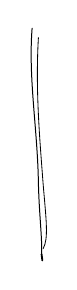
\begin{tikzpicture}[x=1cm,y=1cm,line cap=round]
\draw[line width=.36pt] (0,0) .. controls (-.05,-.64) and (.07,-1.29) .. (.08,-1.97)
 .. controls (.09,-2.38) and (.13,-2.67) .. (.12,-2.87);
\draw[line width=.30pt] (.08,-.12) .. controls (.04,-.79) and (.10,-1.44) .. (.14,-1.98)
 .. controls (.18,-2.45) and (.21,-2.67) .. (.14,-2.80);
\draw[line width=.65pt] (.12,-2.87) -- (.13,-2.95);
\end{tikzpicture}}}
\deleted{\unsure{$\operatorname{Hom}(K$}}
\[
 \Gamma((X,S)/K)\longrightarrow
 \begin{gathered}
 \text{$\pi$-conjugacy classes of}\\
 \text{sections of }\mathcal E\to\Gamma\text{ i.e.}\\
 \text{of sections of }\Pi_1(X)\to\Pi_1(e_K)
 \end{gathered}
\]

\margin{62}

\scanpage{64}
\mspage{30}

is bijective (if $(X,S)$ is an allowed ``anabelian'' pair).
\margin{false as it stands, cf. number 9 below --- one needs additional conditions on the $f$ \ldots\ \uline{Perhaps} \unsure{true if} $I=\varnothing$}

I know in any case that this map is \uline{injective} --- this holds whenever one has a scheme $U$ over $K$ (here $X\setminus S$) which embeds in an \inserted{algebraic group $G$} extension of an abelian variety by a torus, and then follows from the ``absolute'' Mordell-Weil theorem: $G(K)$ is a finitely generated $\mathbb Z$-module.
In fact, it suffices to know the splitting class of the extension $\mathcal E^{\natural}$ of $\Gamma$ by
\[
 \pi_{\mathrm{ab}}=\pi/\overline{[\pi,\pi]}\simeq H_1(\unsure{\mathrm{Alb}|U}),
\]
\deleted{\unsure{to deduce from it}} \inserted{corresponding} to a point of $U$ rational/$K$, to know this point. Thus the \inserted{result of} faithfulness is obtained, with less draconian hypotheses on $X$ than the anabelian hypothesis (with the notation of lemma 5.2, this means that $g=0\Rightarrow\unsure{n|\nu}\ge2$ i.e. that there is no irreducible component of \unsure{$X_{\overline K}$|$U_{\overline K}$} which is isomorphic to \unsure{$\mathbb P^1_{\overline K}$} or $\mathbb E^1_{\overline K}$ \ldots).

\margin{63}

\scanpage{65}

\uline{N.B.} This suggests an approach to the Mordell conjecture, via a better knowledge of extensions of $\Gamma$ by $\pi$: the fact that there is (for $g\ge2$) only a finite number of $\pi$-conjugacy classes of splittings of such an extension \ldots.
Likewise for an approach to Fermat's theorem, via \deleted{\illegible{1}} a good knowledge of an extension of $\Gamma$ by $\pi=\pi_1(\unsure{\mathbb P^1_{\overline{\mathbb Q}}\setminus\{0,1,\infty\}})$ \ldots.

\uline{Case $\overline{\mathrm{IV}}$} $n=1,n'=1$ i.e. $X,X'$ of dimension 1.

a) If $I=I'=\varnothing$, I have nothing to add to the description of morphisms $f:X\to X'$ in terms of morphisms of diagrams of groupoids. Here \deleted{\illegible{1}} the condition $f^{-1}(S)_{\mathrm{r\acute ed}}=S'$ is not a restriction on $f$ --- \deleted{which} one therefore does not exclude constant maps. These (thanks to
\margin{(thanks to \ldots)}
\deleted{If \unsure{$I'\ne\varnothing$} \illegible{5} \unsure{only} $I'=\varnothing$ \inserted{\unsure{i.e. $S'=\varnothing$}} \illegible{7} \unsure{$S'$ is} \unsure{empty}), \unsure{therefore} the condition}

\margin{64}

\scanpage{66}
\mspage{31}

the study \unsure{of the|of the} case \uline{$\overline{\mathrm{II}}$}) are moreover described in a ``fully faithful'' way by homomorphisms of diagrams --- They correspond to the cases $f:\mathcal E'\to\mathcal E$ which are zero on $\pi'$.

b) The case $I'=\varnothing$, $I\ne\varnothing$ (i.e. $S'=\varnothing$, $S\ne\varnothing$) means, for the condition $f^{-1}(S)_{\mathrm{r\acute ed}}=S'$ i.e. $f^{-1}(S)=\varnothing$, that $f$ must map $X'$ into $X\setminus S$, \deleted{One therefore expects} therefore that the $f$ corresponding to a morphism from $(X',\varnothing)$ to $(X,S)$ are constant.
The messy conjecture in this case therefore expresses \deleted{that} essentially that at the level of the homomorphisms $\mathcal E'\xrightarrow{p'}\Gamma$ and $\mathcal E\xrightarrow{p}\Gamma$, every group homomorphism $\mathcal E'\xrightarrow{f}\mathcal E$ such that $pf=\operatorname{int}(\alpha)p'$ for $\alpha\in\Gamma$ [one is reduced to the case where $\alpha=1$, \inserted{$p,p'$ surjective} i.e. to homomorphisms of extensions of $\Gamma$ by \unsure{the|some} groups \unsure{$\pi=\pi_1(\overline{X\setminus S})$} and $\pi'=\pi_1(\overline X')$)] is trivial on $\pi'$ [i.e. ``is'' a section]. One should try to verify this point directly, which (modulo case \uline{$\overline{\mathrm{III}}$}) would establish the ``messy conjecture'' in that case.

\margin{65}

\scanpage{67}

c) The case $I'\ne\varnothing$, $I=\varnothing$ implies that $\operatorname{Hom}((X,S),(X',S'))=\varnothing$ (since $f^{-1}(S)=f^{-1}(\varnothing)=\varnothing\ne S'$ !), which does indeed correspond \deleted{to the case} to $\operatorname{Hom}(\mathcal D',\mathcal D)=\varnothing$ since $\nexists\tau:I'\to I$.

d) In the case $I'\ne\varnothing$, $I\ne\varnothing$, the condition $f^{-1}(S)_{\mathrm{r\acute ed}}=S'$ implies that $f$ is not constant (otherwise one would have $f^{-1}(S)_{\mathrm{r\acute ed}}=\varnothing$ or $X'$), hence $f$ is dominant and finite, generically étale. [Thus, such $f$ \deleted{\unsure{are allowed} \illegible{1}} can occur only if $I$ and $I'$ are either both $\varnothing$ (case a)), or both $\ne\varnothing$ (present case d)). The fact that in these cases, the diagrammatic Galois description is \uline{faithful} (perhaps not fully) follows easily from the analogous result in case \uline{$\overline{\mathrm{III}}$}.
Full faithfulness on the other hand is a mysterious thing, $=$ if the result corresponding \deleted{\unsure{in}} \deleted{\illegible{1}} to case \uline{$\overline{\mathrm{III}}$} were established (\unsure{and from it we}

\margin{66}

\scanpage{68}
\mspage{32}

seem far, $=$ if $K$ finite over $\mathbb Q$ \ldots)

\uline{Elementary} \uline{reductions} To prove the ``messy conjecture'', one is reduced (by finite extensions of the fields $K$) to the case where $\mathcal E\to\deleted{\unsure{K}}\Gamma$ (and, if one insists, also $\mathcal E'\to\Gamma$) is an epimorphism. Unless I am mistaken, knowledge of case \uline{$\overline{\mathrm{III}}$} for finitely generated extensions of $K$, implies the general case for $K$ (with enough technical sweat \ldots).

Returning however to the general case when $\mathcal E\to\Gamma$ is surjective, in every equivalence class of systems $(f:\mathcal E'\to\mathcal E,\alpha\in\Gamma,$ \deleted{\unsure{$f_i$,}} $\tau:I'\to I,$ \deleted{\unsure{$f_{i'}:\mathcal E'_{i'}$}} $(\alpha_{i'}\in\mathcal E_{\unsure{\tau(i')=i}})_{i'\in I'})$, one can find a system with $\alpha=1$, so that $f:\mathcal E'\to\mathcal E$ is compatible with the homomorphisms to $\Gamma$ (i.e. the extension structures).
When one restricts oneself to such systems, \unsure{the|their} equivalence by conjugation is effected by a system \unsure{$(\mu,(\mu_{i'})_{i'\in I'})$} with \uline{$\mu\in\pi$} $(=\operatorname{Ker}p)$, and

\margin{67}

\scanpage{69}

the $\mu_{i'}\in\mathcal E_{i=\tau(i')}$ as before. Thus, $f:\mathcal E'\to\mathcal E$ is \deleted{defined by some} \inserted{a} homomorphism of extensions, defined modulo inner automorphisms by an element of $\pi=\operatorname{Ker}(\mathcal E\to\Gamma)$, and satisfying conditions made explicit elsewhere.
It could be (as we have already remarked) that knowledge of the \deleted{\illegible{1}} $\pi$-conjugacy class of $f$ suffices to determine the ``messy morphism'' into which $f$ fits (if $I,I'\ne\varnothing$).

[This is linked to the question of whether the \deleted{\illegible{1}} \deleted{\unsure{tran}} $\forall d\in\mathbb N^*,\ \operatorname{Trans}_{\mathcal E}(L_i^d,L_i)$ is reduced to $\mathcal E_i$ (where $L_i=\operatorname{Ker}(p_i:\mathcal E_i\to\Gamma)=\operatorname{Im}(\kappa_i:T(\overline K)\to\mathcal E_i)$).
\margin{\deleted{It would suffice that $\operatorname{Transp}(L_i^d,L_i)\cap\operatorname{Transp}(\unsure{\mathcal E}$}}
In that case, $\mathcal E_i$ would be known in terms of $L_i\subset\pi$, and $=$ in terms of the \unsure{rays|kernels} of subgroups that it defines in $\pi$, and a fortiori in terms of the \unsure{rays|kernels} of homomorphisms \unsure{defined} by $\kappa_i:T(\overline K)\to\pi$ \ldots.

\margin{68}

\scanpage{70}
\mspage{33}

\uline{Case where} \inserted{the} $\mathcal E_i\to\Gamma$ \deleted{is} \uline{surjective} (i.e. \inserted{the} \unsure{$k(s_i)=K$} i.e. $s_i$ rational over $K$).
Then, if $(f,$ \deleted{\unsure{$\alpha$,}} $\tau,$ \deleted{\illegible{1}} $(\alpha_{i'}))$ is a homomorphism from $\mathcal D'$ to $\mathcal D$, \deleted{\unsure{for} \illegible{1}} after \deleted{\unsure{modifying}} \inserted{correcting} by $\mu_i\in\mathcal E_i$ having the $=$ image as the $\alpha_{i'}$ in $\Gamma$, \unsure{one may assume} $\alpha_{i'}\in\pi$, in addition to \unsure{$\alpha=1$} (obtained by correcting by a suitable $\mu$).
Thus one describes the homomorphism \inserted{$\mathcal D'\to\mathcal D$} by $(f,1,\tau,(\alpha_{i'}))$, the $\alpha_{i'}\in\pi$. The \deleted{\unsure{systems}} \inserted{condition} \deleted{\illegible{1}} here is that $f:\inserted{\mathcal E'\to\mathcal E}$ be a group homomorphism over $\Gamma$, that \deleted{\unsure{$\operatorname{int}(\alpha_{i'}^{-1})$}} $f(\mathcal E'_{i'})\subset\text{\inserted{$\operatorname{int}(\alpha_{i'}^{-1})$}}(\mathcal E_{\tau(i')=i})$, and that the homomorphism induced \inserted{$\mathcal E'_{i'}\to\mathcal E_i$} by \deleted{\unsure{$f_i=$}} \unsure{$\operatorname{int}(\alpha_{i'})f$|$\operatorname{int}(\alpha_{i'}^{-1})f$} \deleted{\unsure{of $\mathcal E_i$ of}} induces on $T(\overline K)$ (\uline{via} $\kappa_{i'},\kappa_i$) \uline{the homomorphism of multiplication by $d_i$} and nothing more --- how beautiful!
Two systems $(f,\tau,(\alpha_{i'}))$ and $(f',\tau',(\alpha'_{i'}))$ define the $=$ morphism, iff \inserted{$\tau=\tau'$ and if there} exists
\[
 \boxed{\mu\in\pi,\quad\mu_{i'}\in\begin{gathered}L_{i=\tau(i')}\\[-2pt]\rotatebox{90}{$=$}\\[-2pt]\text{\inserted{$\kappa_i(T(\overline K))$}}\end{gathered}}
\]
such that
\[
 f'=\operatorname{int}(\mu)f
\]
\[
 \alpha'_{i'}=\mu_{i'}\alpha_{i'}.
\]

\deleted{\illegible{1}} Let us note that a priori, for $(f,\tau)$ fixed, the $\alpha_{i'}$ are determined modulo right multiplication by elements of $\operatorname{Transp}_{\pi}(\deleted{\unsure{\pi}}(\unsure{L_i^{d_{i'}}},L_i)$,

\margin{69}
